\documentclass[]{article}
\usepackage{lmodern}
\usepackage{amssymb,amsmath}
\usepackage{ifxetex,ifluatex}
\usepackage{fixltx2e} % provides \textsubscript
\ifnum 0\ifxetex 1\fi\ifluatex 1\fi=0 % if pdftex
  \usepackage[T1]{fontenc}
  \usepackage[utf8]{inputenc}
\else % if luatex or xelatex
  \ifxetex
    \usepackage{mathspec}
  \else
    \usepackage{fontspec}
  \fi
  \defaultfontfeatures{Ligatures=TeX,Scale=MatchLowercase}
\fi
% use upquote if available, for straight quotes in verbatim environments
\IfFileExists{upquote.sty}{\usepackage{upquote}}{}
% use microtype if available
\IfFileExists{microtype.sty}{%
\usepackage{microtype}
\UseMicrotypeSet[protrusion]{basicmath} % disable protrusion for tt fonts
}{}
\usepackage[margin=1in]{geometry}
\usepackage{hyperref}
\hypersetup{unicode=true,
            pdftitle={Kruskal--Wallis test cidadania \textasciitilde{} formacao.continuada},
            pdfauthor={Geiser C. Challco geiser@usp.br},
            pdfborder={0 0 0},
            breaklinks=true}
\urlstyle{same}  % don't use monospace font for urls
\usepackage{color}
\usepackage{fancyvrb}
\newcommand{\VerbBar}{|}
\newcommand{\VERB}{\Verb[commandchars=\\\{\}]}
\DefineVerbatimEnvironment{Highlighting}{Verbatim}{commandchars=\\\{\}}
% Add ',fontsize=\small' for more characters per line
\usepackage{framed}
\definecolor{shadecolor}{RGB}{248,248,248}
\newenvironment{Shaded}{\begin{snugshade}}{\end{snugshade}}
\newcommand{\AlertTok}[1]{\textcolor[rgb]{0.94,0.16,0.16}{#1}}
\newcommand{\AnnotationTok}[1]{\textcolor[rgb]{0.56,0.35,0.01}{\textbf{\textit{#1}}}}
\newcommand{\AttributeTok}[1]{\textcolor[rgb]{0.77,0.63,0.00}{#1}}
\newcommand{\BaseNTok}[1]{\textcolor[rgb]{0.00,0.00,0.81}{#1}}
\newcommand{\BuiltInTok}[1]{#1}
\newcommand{\CharTok}[1]{\textcolor[rgb]{0.31,0.60,0.02}{#1}}
\newcommand{\CommentTok}[1]{\textcolor[rgb]{0.56,0.35,0.01}{\textit{#1}}}
\newcommand{\CommentVarTok}[1]{\textcolor[rgb]{0.56,0.35,0.01}{\textbf{\textit{#1}}}}
\newcommand{\ConstantTok}[1]{\textcolor[rgb]{0.00,0.00,0.00}{#1}}
\newcommand{\ControlFlowTok}[1]{\textcolor[rgb]{0.13,0.29,0.53}{\textbf{#1}}}
\newcommand{\DataTypeTok}[1]{\textcolor[rgb]{0.13,0.29,0.53}{#1}}
\newcommand{\DecValTok}[1]{\textcolor[rgb]{0.00,0.00,0.81}{#1}}
\newcommand{\DocumentationTok}[1]{\textcolor[rgb]{0.56,0.35,0.01}{\textbf{\textit{#1}}}}
\newcommand{\ErrorTok}[1]{\textcolor[rgb]{0.64,0.00,0.00}{\textbf{#1}}}
\newcommand{\ExtensionTok}[1]{#1}
\newcommand{\FloatTok}[1]{\textcolor[rgb]{0.00,0.00,0.81}{#1}}
\newcommand{\FunctionTok}[1]{\textcolor[rgb]{0.00,0.00,0.00}{#1}}
\newcommand{\ImportTok}[1]{#1}
\newcommand{\InformationTok}[1]{\textcolor[rgb]{0.56,0.35,0.01}{\textbf{\textit{#1}}}}
\newcommand{\KeywordTok}[1]{\textcolor[rgb]{0.13,0.29,0.53}{\textbf{#1}}}
\newcommand{\NormalTok}[1]{#1}
\newcommand{\OperatorTok}[1]{\textcolor[rgb]{0.81,0.36,0.00}{\textbf{#1}}}
\newcommand{\OtherTok}[1]{\textcolor[rgb]{0.56,0.35,0.01}{#1}}
\newcommand{\PreprocessorTok}[1]{\textcolor[rgb]{0.56,0.35,0.01}{\textit{#1}}}
\newcommand{\RegionMarkerTok}[1]{#1}
\newcommand{\SpecialCharTok}[1]{\textcolor[rgb]{0.00,0.00,0.00}{#1}}
\newcommand{\SpecialStringTok}[1]{\textcolor[rgb]{0.31,0.60,0.02}{#1}}
\newcommand{\StringTok}[1]{\textcolor[rgb]{0.31,0.60,0.02}{#1}}
\newcommand{\VariableTok}[1]{\textcolor[rgb]{0.00,0.00,0.00}{#1}}
\newcommand{\VerbatimStringTok}[1]{\textcolor[rgb]{0.31,0.60,0.02}{#1}}
\newcommand{\WarningTok}[1]{\textcolor[rgb]{0.56,0.35,0.01}{\textbf{\textit{#1}}}}
\usepackage{longtable,booktabs}
\usepackage{graphicx,grffile}
\makeatletter
\def\maxwidth{\ifdim\Gin@nat@width>\linewidth\linewidth\else\Gin@nat@width\fi}
\def\maxheight{\ifdim\Gin@nat@height>\textheight\textheight\else\Gin@nat@height\fi}
\makeatother
% Scale images if necessary, so that they will not overflow the page
% margins by default, and it is still possible to overwrite the defaults
% using explicit options in \includegraphics[width, height, ...]{}
\setkeys{Gin}{width=\maxwidth,height=\maxheight,keepaspectratio}
\IfFileExists{parskip.sty}{%
\usepackage{parskip}
}{% else
\setlength{\parindent}{0pt}
\setlength{\parskip}{6pt plus 2pt minus 1pt}
}
\setlength{\emergencystretch}{3em}  % prevent overfull lines
\providecommand{\tightlist}{%
  \setlength{\itemsep}{0pt}\setlength{\parskip}{0pt}}
\setcounter{secnumdepth}{0}
% Redefines (sub)paragraphs to behave more like sections
\ifx\paragraph\undefined\else
\let\oldparagraph\paragraph
\renewcommand{\paragraph}[1]{\oldparagraph{#1}\mbox{}}
\fi
\ifx\subparagraph\undefined\else
\let\oldsubparagraph\subparagraph
\renewcommand{\subparagraph}[1]{\oldsubparagraph{#1}\mbox{}}
\fi

%%% Use protect on footnotes to avoid problems with footnotes in titles
\let\rmarkdownfootnote\footnote%
\def\footnote{\protect\rmarkdownfootnote}

%%% Change title format to be more compact
\usepackage{titling}

% Create subtitle command for use in maketitle
\providecommand{\subtitle}[1]{
  \posttitle{
    \begin{center}\large#1\end{center}
    }
}

\setlength{\droptitle}{-2em}

  \title{Kruskal--Wallis test \texttt{cidadania} \textasciitilde{}
\texttt{formacao.continuada}}
    \pretitle{\vspace{\droptitle}\centering\huge}
  \posttitle{\par}
    \author{Geiser C. Challco \href{mailto:geiser@usp.br}{\nolinkurl{geiser@usp.br}}}
    \preauthor{\centering\large\emph}
  \postauthor{\par}
    \date{}
    \predate{}\postdate{}
  

\begin{document}
\maketitle

\begin{itemize}
\tightlist
\item
  Report as Word format: \url{kruskal.docx}
\item
  Report as LaTex format: \url{kruskal.tex}
\end{itemize}

\hypertarget{initial-data-and-preprocessing}{%
\subsection{Initial Data and
Preprocessing}\label{initial-data-and-preprocessing}}

R script: \url{kruskal.R} Inital data: \url{data.csv}

\hypertarget{computation-kruskal-wallis-test-and-effect-size}{%
\subsection{Computation Kruskal-Wallis test and Effect
Size}\label{computation-kruskal-wallis-test-and-effect-size}}

\begin{Shaded}
\begin{Highlighting}[]
\NormalTok{(res.kruskal <-}\StringTok{ }\KeywordTok{kruskal_test}\NormalTok{(dat, }\StringTok{`}\DataTypeTok{cidadania}\StringTok{`} \OperatorTok{~}\StringTok{ `}\DataTypeTok{formacao.continuada}\StringTok{`}\NormalTok{))}
\end{Highlighting}
\end{Shaded}

\begin{longtable}[]{@{}lrrrlll@{}}
\toprule
.y. & n & statistic & df & p & method & p.signif\tabularnewline
\midrule
\endhead
cidadania & 92 & 9.3735 & 2 & 0.0092 & Kruskal-Wallis &
**\tabularnewline
\bottomrule
\end{longtable}

\begin{Shaded}
\begin{Highlighting}[]
\NormalTok{(ezm <-}\StringTok{ }\KeywordTok{kruskal_effsize}\NormalTok{(dat, }\StringTok{`}\DataTypeTok{cidadania}\StringTok{`} \OperatorTok{~}\StringTok{ `}\DataTypeTok{formacao.continuada}\StringTok{`}\NormalTok{, }\DataTypeTok{ci =} \OtherTok{TRUE}\NormalTok{))}
\end{Highlighting}
\end{Shaded}

\begin{longtable}[]{@{}lrrrrll@{}}
\toprule
.y. & n & effsize & conf.low & conf.high & method &
magnitude\tabularnewline
\midrule
\endhead
cidadania & 92 & 0.0828 & 0.0029 & 0.23 & eta2{[}H{]} &
moderate\tabularnewline
\bottomrule
\end{longtable}

\hypertarget{post-hoc-tests-pairwise-comparisons}{%
\subsection{Post-hoc Tests (Pairwise
Comparisons)}\label{post-hoc-tests-pairwise-comparisons}}

\begin{Shaded}
\begin{Highlighting}[]
\NormalTok{pwc <-}\StringTok{ }\KeywordTok{dunn_test}\NormalTok{(dat, }\StringTok{`}\DataTypeTok{cidadania}\StringTok{`} \OperatorTok{~}\StringTok{ `}\DataTypeTok{formacao.continuada}\StringTok{`}\NormalTok{, }\DataTypeTok{detailed=}\NormalTok{T, }\DataTypeTok{p.adjust.method =} \StringTok{"bonferroni"}\NormalTok{)}
\KeywordTok{add_significance}\NormalTok{(pwc)}
\end{Highlighting}
\end{Shaded}

\begin{longtable}[]{@{}lllrrrrllll@{}}
\toprule
.y. & group1 & group2 & n1 & n2 & estimate & statistic & p & method &
p.adj & p.adj.signif\tabularnewline
\midrule
\endhead
cidadania & Doutorado - Concluído & Formação continuada - Concluída & 28
& 46 & -7.7081 & -1.2079 & 0.2271 & Dunn Test & 0.6813 &
ns\tabularnewline
cidadania & Doutorado - Concluído & Formação continuada - Em andamento &
28 & 18 & -24.4762 & -3.0430 & 0.0023 & Dunn Test & 0.007 &
**\tabularnewline
cidadania & Formação continuada - Concluída & Formação continuada - Em
andamento & 46 & 18 & -16.7681 & -2.2654 & 0.0235 & Dunn Test & 0.0705 &
ns\tabularnewline
\bottomrule
\end{longtable}

\hypertarget{report-kruskal-wallis-test-with-plots-and-descriptive-statistic}{%
\subsection{Report Kruskal-Wallis test with Plots and Descriptive
Statistic}\label{report-kruskal-wallis-test-with-plots-and-descriptive-statistic}}

\begin{Shaded}
\begin{Highlighting}[]
\KeywordTok{get_summary_stats}\NormalTok{(}\KeywordTok{group_by}\NormalTok{(dat, }\StringTok{`}\DataTypeTok{formacao.continuada}\StringTok{`}\NormalTok{), }\DataTypeTok{type =}\StringTok{"common"}\NormalTok{)}
\end{Highlighting}
\end{Shaded}

\begin{longtable}[]{@{}llrrrrrrrrr@{}}
\toprule
formacao.continuada & variable & n & mean & median & min & max & sd & se
& ci & iqr\tabularnewline
\midrule
\endhead
Doutorado - Concluído & cidadania & 28 & 2.815 & 2.667 & 1.333 & 4.500 &
0.616 & 0.116 & 0.239 & 0.667\tabularnewline
Formação continuada - Concluída & cidadania & 46 & 2.656 & 2.500 & 1.000
& 4.333 & 0.797 & 0.117 & 0.237 & 1.167\tabularnewline
Formação continuada - Em andamento & cidadania & 18 & 2.213 & 2.167 &
1.500 & 3.333 & 0.568 & 0.134 & 0.283 & 0.792\tabularnewline
\bottomrule
\end{longtable}

\begin{Shaded}
\begin{Highlighting}[]
\KeywordTok{kruskal.plot}\NormalTok{(dat, }\StringTok{"cidadania"}\NormalTok{, }\StringTok{"formacao.continuada"}\NormalTok{, res.kruskal, pwc, }\KeywordTok{c}\NormalTok{(}\StringTok{"jitter"}\NormalTok{))}
\end{Highlighting}
\end{Shaded}

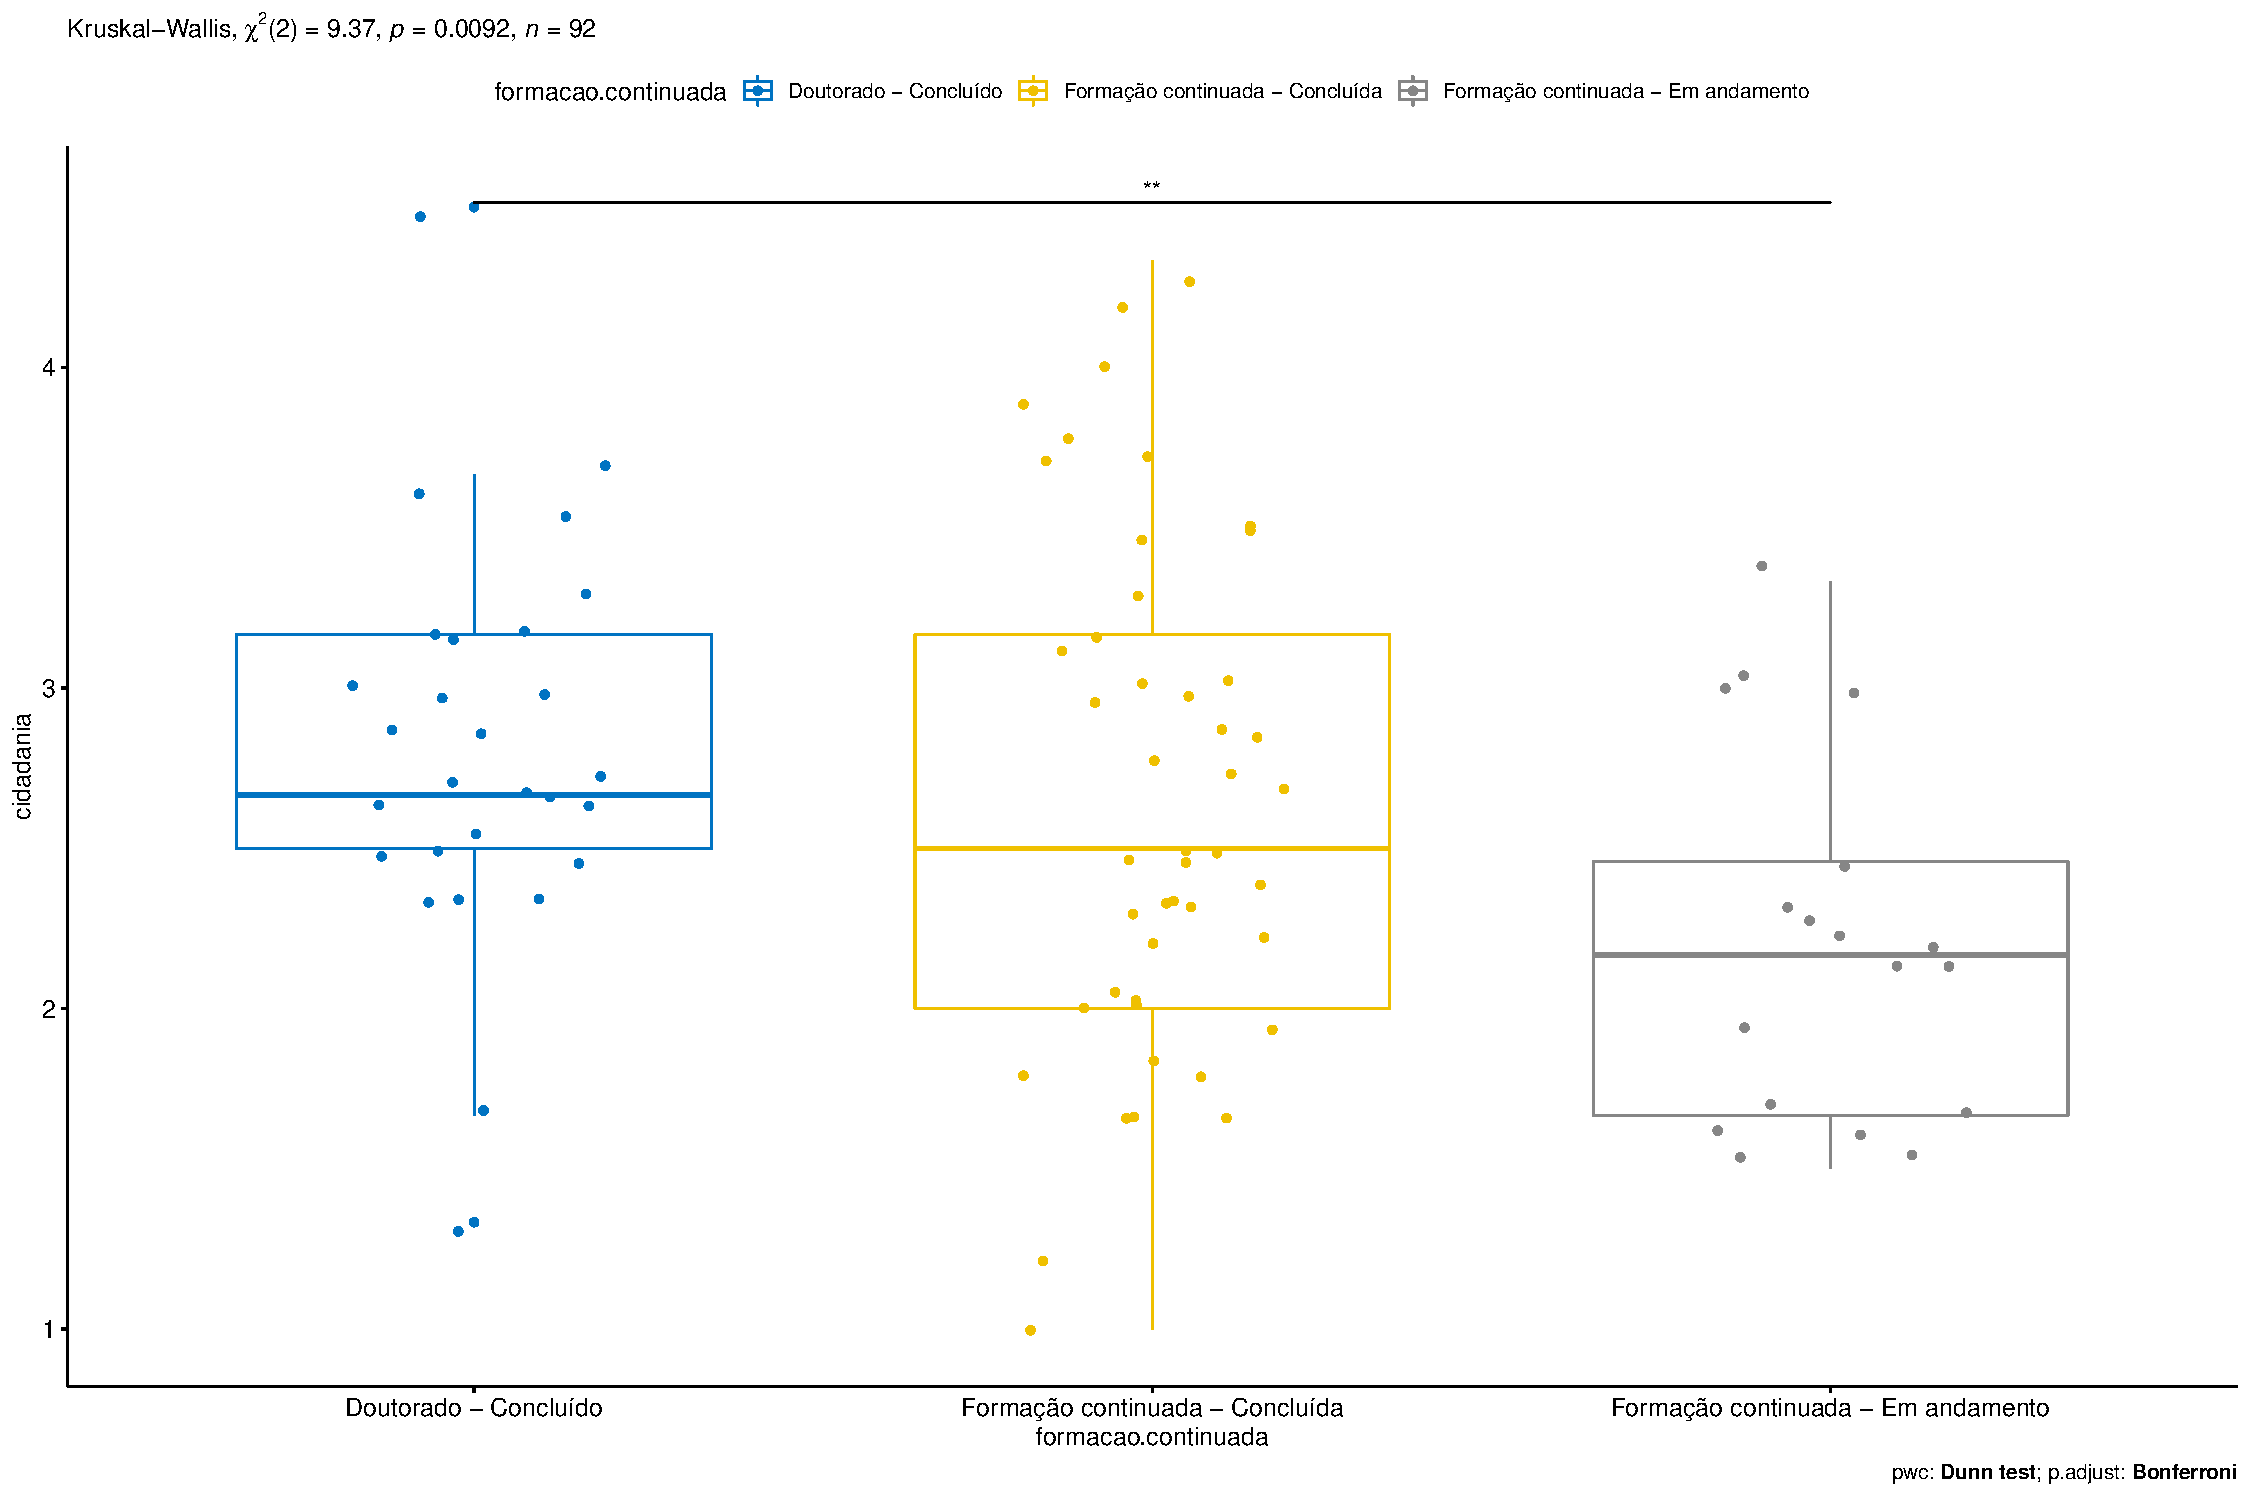
\includegraphics{kruskal_files/figure-latex/unnamed-chunk-5-1.pdf}


\end{document}
